Dans ce chapitre, nous allons aborder les aspects techniques liés au développement de notre application.

\section{Le format de fichier ``.snake''}
Les différents snakes proposés par l'application sont stockés dans des fichiers ``*.snake'' dans le répertoire ``Snakes''. Le listing~\ref{.snake} ci-après montre le contenu du fichier ``snake.snake'' soit le serpent chargé par défaut par l'application.\newline

La section \verb|[Volume]| permet de définir les caractéristiques du volume final, soit :
\begin{itemize}
 \item sa largeur (x);
 \item sa hauteur (y);
 \item sa profondeur (z);
 \item l'état de chacun des sous-cubes le formant (x;y;z;State).
\end{itemize}

La première ligne indique les dimensions (maximales, sur les trois axes) du volume final. L'exemple présenté ici indique que le volume à remplir est contenu dans un cube de 3x3x3. 
Ensuite, on associe à chaque triplet de coordonnées un ``état'', matérialisé par la dernière valeur entière de chaque ligne. La valeur 1 signifie que le volume final occupe l'espace à cette coordonnée. La valeur -1 indique au contraire que le volume final ne doit pas occuper cet emplacement.\newline

La section \verb|[Snake]| définit le nombre et l’enchaînement des unités formant le serpent. La valeur 0 indique que l'unité est une extrémité du serpent, la valeur 1 indique une unité de type ``droite'' et la valeur 2 une unité de type ``angle''.\newline

La section \verb|[Symetry]| permet quant à elle de définir quels sont les axes de symétrie à prendre en compte lors de la recherche des vecteurs initiaux (cf partie 3.4). La valeur 1 représente le fait qu'un axe de symétrie est applicable aux faces du volume tandis que la valeur 0 indique qu'il ne convient pas de l'utiliser. Ces quatre entiers correspondent respectivement aux axes de symétrie vertical, horizontal, diagonal anti-slash et diagonal slash.

\newpage
\begin{lstlisting}[caption=Contenu du fichier snake.snake]
 [Volume]
  3;3;3
  0;0;0;1
  0;0;1;1
  0;0;2;1
  0;1;0;1
  0;1;1;1
  0;1;2;1
 
  [ ... ]
 
  2;1;1;1
  2;1;2;1
  2;2;0;1
  2;2;1;1
  2;2;2;1
  [Snake]
  27
  0;1;2;2;2;1;2;2;1;2;2;2;1;2;1;2;2;2;2;1;2;1;2;1;2;1;0;
  [Symetry]
  1;1;1;1
\end{lstlisting}\label{.snake}

\section{L'utilisation des threads}
Nous avons dès le départ pris le parti d'utiliser la technique du multithreading afin de séparer l’exécution du rendu 3D et le reste de l'application. Cela permet notamment de faciliter la gestion des animations et, de manière plus générale, de limiter la dépendance du rendu 3D avec les diverses fonctions de calcul. 

Plus tard dans le développement de l'application, nous avons étendu l'utilisation des threads au calcul des solutions. Cette parallélisation a permit d'améliorer le temps de calcul, en particulier pour le Snake Cube de taille 4x4x4.\newline

Le schéma suivant (Fig.\ref{threads}) montre l'organisation des threads de notre programme. On distingue 4 types de threads :
\begin{itemize}
 \item Le thread principal, qui a pour rôle de créer les autres thread et qui fait donc office de thread de contrôle. C'est également lui qui se charge de l’interaction homme/machine (récupération et interprétation des entrées clavier/sourie).
 \item Le thread graphique à qui il incombe d'actualiser l'écran de sorte à avoir dans l'idéal une fréquence de 60 images par seconde. Ce thread est démarré au lancement du programme et se termine lors de la fermeture du l'application.
 \item Le thread de calcul, dont le rôle est de répartir le travail de recherche des solutions au différents threads de résolution de noeud. Se thread permet de calculer les solutions pour un snake tout en laissant la possibilité à l'utilisateur d'interagir avec l'application (pression sur la touche ``échap'' notamment. Ce thread est démarré en mode détaché pour recherché toutes les solutions lorsque l'utilisateur charge un nouveau serpent. Il peu également être lancé en mode attaché (attente de la fin de l’exécution) lorsque l'utilisateur demande une aide à la résolution. Ce démarrage en mode attaché représente une contrainte que nous n'avons pas eu le temps de contourné. En effet, quand ce thread est en mode attaché, il perd sa capacité à totalement paralléliser le travail de recherche. L'utilisateur ne peut donc plus interagir avec l'application pendant le calcul, le thread principal étant bloqué par l'attente de la fin de l'exécution du thread de calcul.
 \item Les thread de résolution de noeud; ces threads sont créés par le thread de calcul. Il permette d'explorer plusieurs branche de l'arbre de recherche en même temps, permettant ainsi de réduire le temps de calcul. Le nombre de point de départ (de branches) à explorer pour chaque thread de résolution de noeud est définit de la manière suivante : soit n le nombre de thread de résolution de noeud à utiliser et x le nombre de point de départ possible pour résoudre le snake. Le nombre de point départ affectés au n-1 premier thread sera a = x / n. Pour le n\up{ième} thread, le nombre de point de départ affectés sera b = n - ((n-1) * a). Nous verrons dans la partie ``Résultats'' que cette façon de faire présente un inconvénient.
\end{itemize}

\begin{figure}[h]
 \centering
 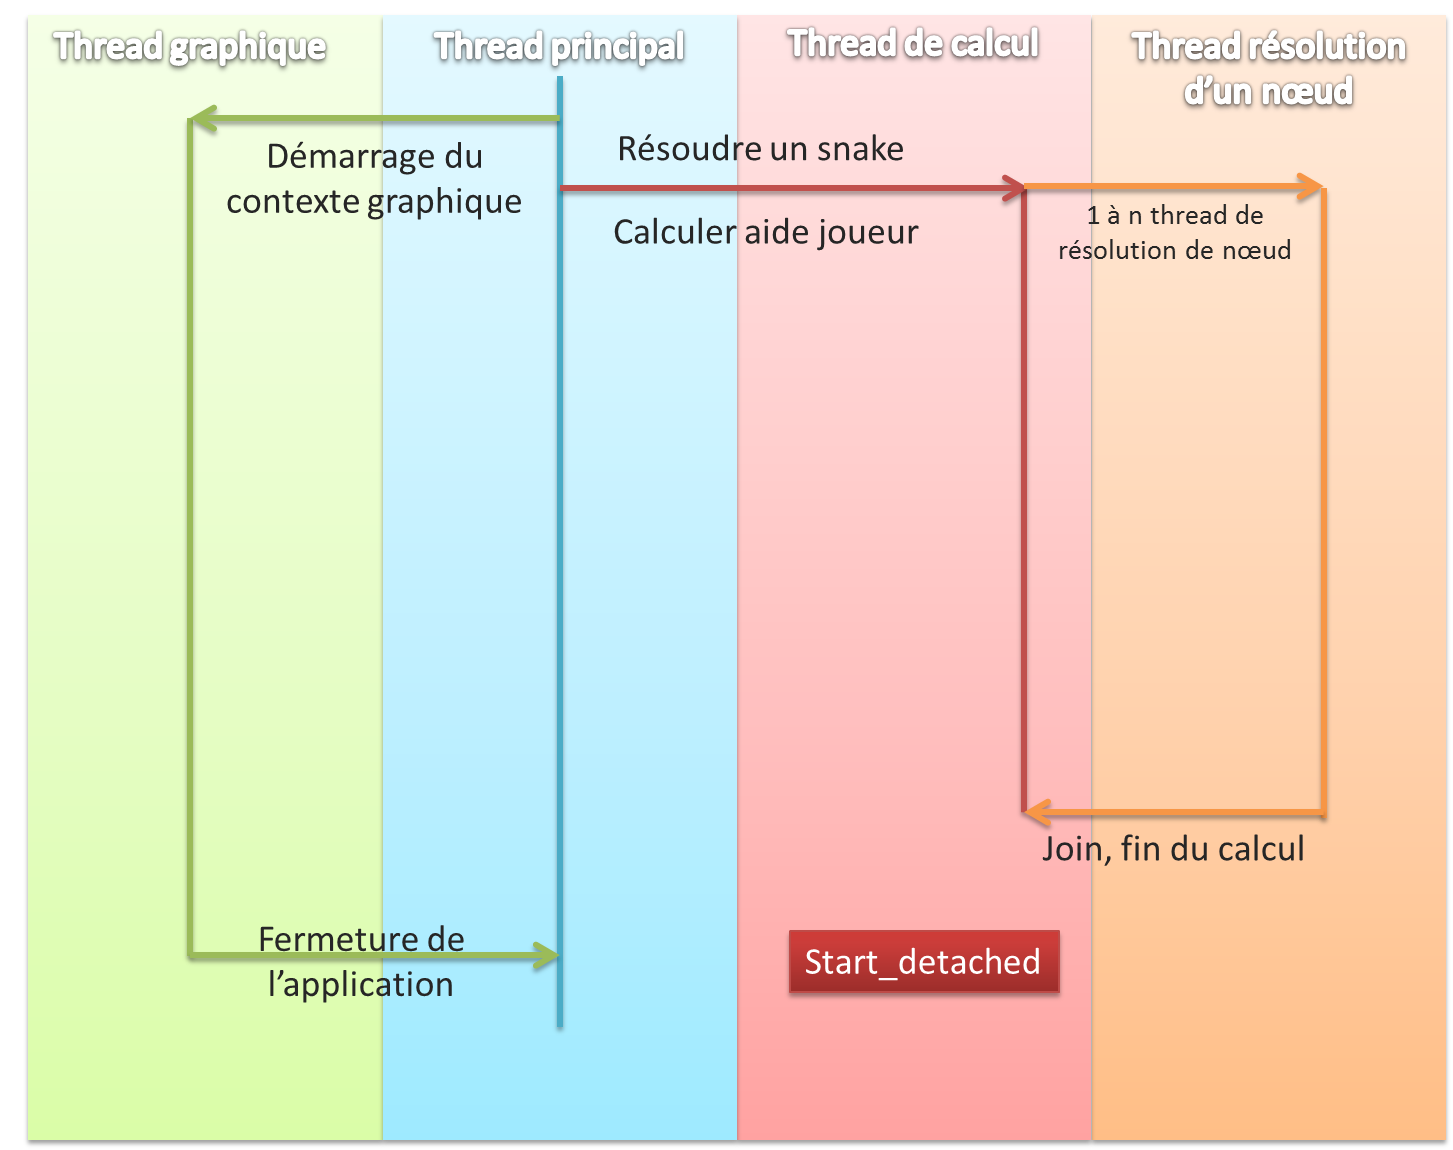
\includegraphics[scale=0.4,keepaspectratio=true]{img/threads.png}
 \caption{Organisation des threads}
 \label{threads}
\end{figure}